\section{Introduction}
% Just here to show that we can put todo notes in the doc, can be removed later
% Let's do things\todo{sup}

% Just here to show how listings are done in this template, can be removed later
% \begin{lstlisting}
% test
% fiets
% test
% \end{lstlisting}

% Short abstract introduction here about this section (can be done when finished)

\subsection{Background}
\label{introduction-background}
% What is SeaDataCloud's exact problem? Make the problem clear so that our solution fits the problem. Try to look at it from all angles, like an os3 teacher would
% SeaDataCloud is a distributed infrastructure to manage large and diverse sets of data about seas and oceans. This Pan-European network offers data access to support scientific workflows which varies from climate change prediction to offshore engineering\cite{sdc}. SeaDataCloud has 8 institutes with over 100 data centers, with the aim to make research data available to scientist.

% Different independent organizations push data into this infrastructure which are then automatically and manually curated to ensure correct data formats. A PID (Persistent Identifier) is then assigned when it’s stored in the catalog. This PID ensures that the data can be identified, independent of its location in the infrastructure\cite{icn-survey, icn-bd}.

% Data consumers pull data from this catalog by the means of point-to-point connections (IP), where every data request from the consumer are answered with a data transfer from the source (the producer). This approach can potentially cause congestion and delays with many data consumers. Named Data Networking (NDN) is a data centric approach where unique data, once requested, is stored on intermediate locations. Consecutive requests for that unique data object are then made available by these intermediate locations (caching). This approach distributes traffic load more efficient and reliable compared to point-to-point connection oriented techniques\cite{ndn}.

Having access to marine data is of vital importance for marine research and a key issue for various studies, which varies from the climate change prediction to off shore engineering.
SeaDataNet connects together more than hundred data centres from eight European marine institutes in different geographical domains, aiming at preserving and making re-useable marine observations ranging from ocean physics to chemistry and biology. 
It is a distributed marine data infrastructure network for managing the large and diverse data sets collected by the oceanographic fleets and the automatic observation systems.
SeaDataNet started the SeaDataCloud project in 2016 (and lasts till 2020), aiming at considerably advancing SeaDataNet Services and increasing their usage, adopting cloud and high performance computing technology for better performance \cite{sdc}.

SeaDataClouds current model is a centralized solution, as the current cache is a central catalogue which duplicates the entire data repository. Data consumers use host-to-host-connections to pull data from this cache. This can cause a lot of congestion with many data consumers and does not distribute load efficiently. 

SeaDataCloud proposed a model to introduce NDN, as seen in figure \ref{fig:sdc_ndn}. With NDN, data is cached at intermediate routers which brings the data closer to the consumer. The data hosting organization pushes the object in NDN, where the PID resolver does the translation from PID name to a NDN name (to be used within NDN) and inserts the data in NDN. After the object has been inserted in NDN, the data consumer can then request the object from the NDN network.
Their proposed model currently only supports one PID provider also referred to as a PID type. Interoperability between different PID types within NDN has not been realized yet at SeaDataCloud..

\begin{figure}[H]
\centering
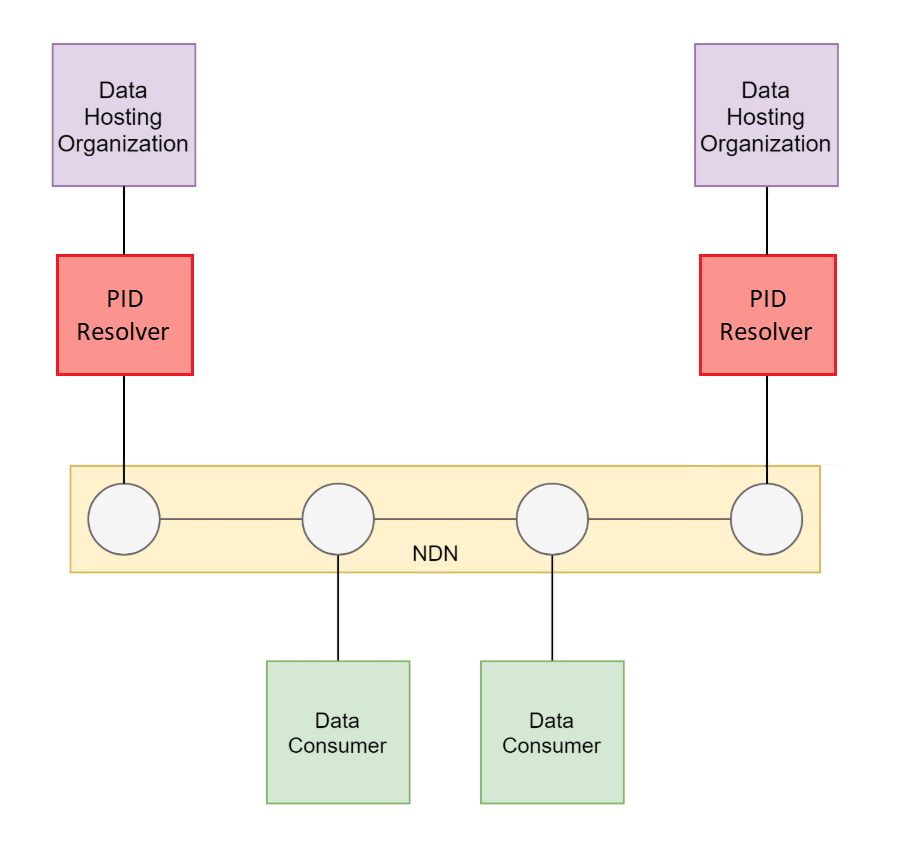
\includegraphics[scale=0.4]{Images/sdcrp2.png}
\caption{SeaDataClouds proposed NDN model.}
\label{fig:sdc_ndn}
\end{figure}

\subsection{What is a PID?}
Shortly after the introduction of the WWW, Tim Berners Lee (its creator) proposed in the IETF to use the Uniform Resource Identifier (URI) as the naming scheme for identifying 
contents on the Web. This proposal got rejected by IETF, due to the fact that it does not allow users of the Web to change the URI of the Web contents when moving the Web contents to another location. This lead to the use of Uniform Resource Locators (URLs) as the naming scheme to identify Web content. In this paper, the term Web content refers to a digital object.
 
The use of URLs was no issue at the early stages of the Web, but after a while users of the Web began to experience the problem of a broken link, or the so called "link rot" problem, 
where a user fails to retrieve the digital object by its URL, 
due to the fact that the location of the digital object has been changed \cite{icn-bd, ark-id}. 

Therefore the first PID systems emerged in the mid-1990s shortly after the introduction of the Web itself. 
A PID is a long-lasting, permanent reference to a digital object. Traditional identifiers, such as the bibliographic identifier ISBN will not be interpreted as a 
hyperlink by Web browsers. For example the string \texttt{ISBN 951-45-9942-X} has to be expressed as a HTTP URI in the form of \texttt{http://urn.fi/URN:ISBN:951-45-9942-X} to be a persistent link to the resource.  
When using a PID, a user who requests the digital resource can trust that the appropriate digital resource is retrieved, even if the location where it resides has been changed \cite{pid-oview}.

\subsection{What is NDN?}
When the internet was conceived it was designed for host-to-host communication. This means that in order to retrieve data, a host needs to retrieve its data from a single source. Nowadays the internet is increasingly data-oriented rather than host-oriented. For example, in 2018 15\% of the worldwide average bandwidth use was consumed by Netflix, with regional peaks often reaching 40\% \cite{introduction-netflix}. With many users requesting the same video, congestion becomes a problem. The geographical location sits on top of that problem, since data needs to cross distance as well, resulting in latency. When Netflix users request the same content, then the content would be downloaded once from the Netflix servers and then cached in NDN. Consecutive request would then retrieve the content from the nearest NDN cache rather from Netflix itself. This alleviates network latency and congestion.

The primary use case of the internet has become data distribution. Solving distribution problems with a host-to-host communications network is complex and error prone. The focus of NDN \cite{ndn-summary} is to change the communication model by removing the restriction that packets can only name communication endpoints. In an NDN network the endpoint is a chunk of a video, book or data set.

NDN’s minimal functionality includes support for consumer-driven data delivery, built-in data security, and use of in-network caching. This model provides support for scaling data, balancing data flows for congestion control and retrieving data via multiple paths. This is done by routing packets based on their name rather than destination. When data is sent across the NDN network, it's cached at intermediary hops. Consecutive request for the same data can then be provided by these local in-network caches. If Netflix would apply NDN, then popular content would be cached on intermediary hops. The data integrity can be verified via cryptographic hashes. Therefore, this data-oriented model mediates congestion and latency compared to host-oriented models. Section \ref{overview-ndn} provides a more detailed explanation of NDN.

\subsection{Related work}
\label{introduction-related-work}
% Related work summary, only stuff that's directly relevant for our research. Other references can be made later by simply mentioning them. Avoid summarizing related work in too much detail, keep it clear and concise. We need to show our contribution, not what others did.

% short intro about this section needed, connecting the pid and ndn part
In this section...

\subsubsection{PID interoperability}
In 2014, Karakannas researched the efficiency of ICN for delivering big data with PIDs. PIDs are used in big data infrastructures to identify digital content and research data. An example of a PID type is DOI (Digital Object Identifier), which is used for object identification. In section \ref{pid-types} we will explain more about PID types. The research proposed a mapping architecture for resolving PIDs to ICN names. Karakannas proposed to use a PID to NDN mapping server for every PID type instead of doing the translation on the clients browser. For the latter the researcher states that translation of a PID to NDN name will be highly depended on the clients NDN browser which will need to be updated every time a new rule would be appeared or changed \cite{icn-bd}.
%The research results showed that in-network caching can offer significant performance benefits, when the cache size of the network elements that perform in-network caching is bigger than the Big Data object size. 

In 2017, Mousa researched the fetching and sharing of DOI objects with information centric networking paradigm such as NDN. 
%(Named Data Networking). 
%For this, the effect of ordering a group of objects in ascending or descending order according to their sizes before requesting them one by one was studied. The research concluded that these ordering methods showed that the methods proposed can dramatically influence the fetching performance of objects from NDN networks. 
The researchers approach focused only on DOI identified objects within NDN networks, which was possible, and states that there are many other different PID systems that can also be integrated. Furthermore, the researcher explains that difference in NDN naming of different PID providers must be taken into account, such that the correct prefix is used within NDN to identify specific PID types within the NDN network. For example using the prefix \texttt{"doi/"} within NDN for DOI identified objects. 
%By doing this,   
In the researchers' model, the translation happens at the consumers browsers and a consumer has the choice to either request the digital object by its NDN name or PID \cite{ndn-app-aware}.
%Rahaf Mousa also experimented with cache replacement methods to evaluate which method gives the most performance gain and found that LRU (Least Recently Used) cache replacement strategy gives the highest performance with the proposed ascending ordering according to size method \cite{ndn-app-aware}.

Zhao et al. progressed the research done by Karakannas and Mousa and proposed an architecture to map PIDs onto the naming scheme of NDN. Their proposed solution is called NDN-as-a-service for PID data objects (NaaS4PID) and supports one PID type. This solution is composed out of three key components \cite{icn-resteam}:
\begin{itemize}
  \item PID2NDN gateway; primarily responsible for resolving PIDs to NDN names.
  \item NDN4PID router image; an NDN node that implements a virtualized NDN router.
  \item NDN4PID manager; automates the management of the NDN overlay in\newline cloud or e-infrastructure.
\end{itemize}

Olschanowsky et. al. looked into translating climate modeling scheme filenames, used by CMMAP applications at Colorado State University, to a name usable in NDN. The researchers designed a NDN name translator to support the data management needs of CMMAP. The NDN name translator incorporates a naming schema that is designed to be compatible with existing climate modeling schemas, like CMIP5, while allowing for some flexibility for project-specific requirements. 
They explain that NDN names for climate data should be both expressive and human readable. The advantages of long expressive names versus short easy to remember names have to be balanced.
The researcher state that every data provider should publish a data prefix which acts as a globally
routable prefix within NDN covering all of the data made available by the
provider. This complies with Mousa, who stated that NDN naming of different PID providers must be taken into account.
The researchers consulted with CMMAP climate scientists and confirmed that these naming rules are acceptable for their datasets and are appropriate for global distribution. 
However, the translation is not as easy as taking the filename only and translating it into a NDN name. To construct a usable NDN name to uniquely identify data of a specific model, the filename to NDN translator has to parse file metadata or even glean in the data itself to mine for missing name components. 
For example the CMMAP name \texttt{"spcesm-ctrl.pop.h.1891-01.nc"} translates into \texttt{"/coupled/control/CMMAP/spcesm-ctrl/pop/1M/1891-01/"}. In this example it is shown that after the prefix identifying the provider \texttt{"/coupled/control/CMMAP/"}, the NDN translated name contains additional information next to the filename, which is parsed from metadata or information that resides in the data itself \cite{ndn-clim}.

% TO-DO
%The research done by Fan et. al. utilizes a catalog which 
%-Almost same model as us, catalog instead of GW
The research done by Fan et. al. utilizes a catalog which holds the the translation of NDN names. Users query the catalogue to receive a NDN name. This process is fairly lightweight since the catalog need only concern itself
with the addition/removal of names rather than heavyweight
dataset synchronization.
The researchers use datasets of the CMIP5 climate modeling scheme for their research and encourage to use the climate modeling scheme as a prefix for a NDN name. 
Their catalog design can support the needs of any community, which can be seen as a data provider described earlier, that is able to define and use consistent naming schemes.
The researchers conclude that their catalog facilitates NDN name discovery and that data management can be made easier for scientific communities as long as they converge on common naming schemes \cite{ndn-man}. 

\subsubsection{NDN performance and scalability}
\label{introduction-related-work-ndn}
ICN is the common architectural idea of forwarding packets based on their name rather destination (TCP/IP). Research done by Karakannas \cite{icn-bd} concluded that NDN was the only ICN approach that published a specification and workable software to experiment with. As of writing this report, we concluded that this conclusion still holds up. Therefore, this research used NDN for experimentation.

James McCabe's "Network Analysis, Architecture, and Design" \cite{mccabe2010network} book offers a systems methodology approach towards network design. The approach is described in McCabe as "seeing the network part of a larger system, with interactions and dependencies between the network and its users, applications and devices". The methodology put forward by McCabe is to design a network based on several inputs and outputs:
\begin{itemize}
    \item Analysis: What do users/services require? How are the relationships composed between these components?
    \item Architecture: Which technology and topology choices support the users/services needs? Based on this, create high-level, end-to-end structure of the network.
    \item Design: Determine the physical detail of the architecture based on output of previous steps.
\end{itemize}

The inputs and outputs used in this method are intended to be iterative and by no means define a final architecture design. This is due to the fact that requirements, technology and user behaviour can change and with that the network design. Section \ref{overview-mccabe} provides a more detailed overview of this method and section \ref{planning-ndn} describes how it's applied for this research.

NDN is relatively new and thus not much is known yet about the performance in different scenarios. In order to plan a network, it would be necessary to know what works and doesn't work for NDN. Large NDN testbeds are still rare. However, there is sufficient research available that focused on particular design choices of NDN. Research done by Lim et al. \cite{lim2018ndn} at a large existing testbed located in the USA \cite{ndn-testbed-status} highlighted a few lessons learned. Lim et al. setup the first intercontinental NDN testbed with the intent to see the benefits for big science (big data). They implemented a name translator for climate-science data, which translated CMIP files to an NDN compatible name. They concluded that NDN provided performance improvements compared to classical climate data delivery techniques based on TCP/IP. A network was used for testing which provided direct links across the USA. The research concluded that NDN over UDP does not properly support large NDN packets (> 64kB). According to the research this was due to UDP's properties of not applying congestion control and proper packet retransmission and resulted in unsatisfying performance. The loss of a single UDP segment resulted in the retransmission of a large NDN data packet, consisting out of many UDP packets. However, NDN over TCP demonstrated a more reliable and faster performance due to the allowance of larger dynamic window sizes and congestion control. Native NDN congestion control is still an open research area \cite{ren2016congestion}, as of writing this report, no proposal has been implemented.

The performance benefits of NDN concluded by Lim et al. correlates with research done by Shannigrahi et al. at the USA-based large hadron collider network \cite{shannigrahi2015named}. Shannigrahi et al. achieved a 71\% reduction in the average delay per data chunk compared to a no-caching case. Shannigrahi et al. conducted NDN caching simulations \cite{shannigrahi2017request}. They concluded that a small cache of several gigabytes already reduces network load. However, as expected, increasing the cache towards 1TB reduced the network load even more. However, this reduction of load wasn't proportional with the cache size. They concluded in their research that a 1GB NDN cache at the edge of the NDN network can already significantly improve data distribution and reducing the network load from servers. The average file size in use was 1.3GB.

Furthermore, in NDN several caching, cache replacement and forwarding strategies can be used to fine-tune performance. Koulouzis et al. researched these strategies and concluded that the "leave copy everywhere" caching strategy provided the best performance ratio between cache size to data object size for generic data usage. However, "leave copy down" and "leaving copies with probability" performed best for delivering big data objects. Koulouzis et al. also concluded that the ascending ordering of data objects enhances network performance when combined with the "least recently used" caching strategy. This was concluded based on observations that if large objects were requested first, the cache replacement algorithm would make room by overwriting files already in the cache, resulting in cache misses. When small files were requested first, more cache hits were measured. As for cache size, the researchers recommended a cache size at least twice the size of the biggest data object in the network. Yuan et al. \cite{yuan2012scalable} researched the performance of NDN forwarding. They used the CCNx application to perform experiments. Their research concluded that packets with long names degraded performance. After profiling the software they measured that the NDN name decode operation took 35.46\% of the entire program running time. So et al. \cite{so2013named} goal was to develop a method to have fixed lookup times with variable length names. In order to achieve this goal they explored hash tables to do name lookup. On top of that they explored the possibility to do this in hardware by using a Cisco ASR9000 router with the integrated service module. This module ran 64-bit Linux, using 2 Intel 2.0GHz hexa-core Westmere EP (Xeon) processors with hyper-threading. Additionally it included up to three 2TB SSD drives. With their experiments they managed to forward 20Gbps of real NDN traffic. Research done by Tortelli et al. \cite{tortelli2013performance} researched the effectiveness of two opposite forward strategies; flooding and best-route (with and without caching). Several experiments let them to the conclusion that there are pros and cons in each forwarding strategy, but that it's difficult to determine an overall well performing forward strategy.

\subsection{Research question}
% Based on the use case and related work, what is it that we will research and why? What is it that we want to answer?
In this section we will formulate our research question based on SeaDataClouds proposed model to achieve interoperability between different PID providers to uniquely identify digital objects in NDN. Next to this, we look into using NDN to cache digital objects closer to the data consumer to reduce latency and congestion, instead of using a centralized cache which duplicates the entire data repository. For using PIDs in NDN, we have to look into PID to NDN translation to make PIDs interoperable in the NDN network. Therefore the following research question is formulated.

\begin{itemize}
	\item How to make the Persistent Identifier (PID) and NDN (Named Data Networking) namespace interoperable?
\end{itemize}

As SeaDataClouds proposed solution only supports one PID type at the moment, we will look into supporting different PID types to find a feasible solution to implement future PID types easily. This will be answered with the following subquestions.
\begin{itemize}
    \item[--] How to support different PID types?
    \item[--] How to incorporate extensibility for future PID schemes?
\end{itemize}

As SeaDataClouds current model is a centralized solution, which can cause a lot of congestion with many users and does not distribute load efficiently and reliably, their proposed model incorporates NDN to overcome the issues of traditional host-to-host oriented techniques. Therefore we will be looking into introducing NDN in SeaDataCloud. To achieve this, the following research question needs to be answered.   
\begin{itemize}
    \item How to plan and scale an NDN network?
\end{itemize}

An important aspect is to efficiently use an NDN network in such a cloud infrastructure by scaling up or down to adapt to the load. To accomplish this, 
%we will look into 
%To plan and scale an NDN network, 
the known NDN scaling problems must be analyzed. Furthermore, we will look into methods to make it possible to plan and scale an NDN network by deploying (orchestrating) components of an NDN network in a SDN-like way.
\begin{itemize}
    \item[--] Which NDN scaling problems are known?
    \item[--] Which method can be used to plan an NDN network?
    \item[--] How to deploy an NDN network in a scalable way?
\end{itemize}


\subsection{Scope}
% What will we do and what will we skip? Based on what's already done in related work and our research question
% The use case that SeaDataCloud offers is suitable to further research and improve interoperability of different PID types in NDN and planning and scaling such an NDN network. In order to accommodate multiple data producers, for which each has their own PID scheme, a custom tailored mapping needs to be made which will be derived and from the related work done earlier and improve our model by tackling the issues the researches came across. Support for future PID types with different naming schemes should be easily extensible, therefore we will also look into a solution which makes this possible. 

% This also requires to look into the design patterns of such a deployment where scalability and automated provisioning are key requirements. For this, we will look into different solutions like Kubernetes and TOSCA for managing an NDN network in a Software Defined Networking (SDN) fashion.

Based on related work and the research question we defined the following scope for our research. For this research and our experiment, we will make the PID types URN, Handle and DOI interoperable with the NDN namespace to show that interoperability of different PID types is possible within NDN.
%that it is possible to make different PID types interoperable within the NDN namespace.
The reason we do not cover more PID types in our experiment, is because with the aforementioned PID types we can already prove that PID interoperability is possible. There are more PID types than the most widely ones in use, it is up to the the PID providers which are used within SeaDataCloud to add the PID types they provide. We also aim to define a solution where future PID types can be added easily.
Therfore, the interoperabilty goals are to show that different PID types can be used within NDN and delivering a method to easily support new PID types, which can be proven with a few PID types.

%that future PID types can be added easily, and not to add as many PID types in our experiment.

%and PID Y will be made interoperable with NDN. PID A and PID B are not done because of 'reasons', be specific about this (a no-no is saying that we don't have enough time, real reasons, show that we've thought about this). This goal entails having this and that end result.

The planning of the NDN network has the following goals. Based on known performance limitations and the SeaDataCloud use case we will create a method for planning and deployment. This will include a proof of concept where, based on certain NDN parameters, the network can be adjust for scale. For ease, these parameters need to be centrally controlled and compatible with different cloud providers. Support for different cloud providers is needed for flexibility, this broadens the choice for cloud providers.

\subsection{Report structure}
To-do after finishing our paper.

%After having introduced the reader to the concepts and related work of our researched subjects, this paper starts with a technical overview of the technology being used in section \ref{tech-oview}. In this section we will describe PIDs, NDN, McCabem, TOSCA and virtualization in more depth and more detail.
%The paper continues by describing our methodology in section \ref{method}, which includes showing our proposed model which describes how interoperability is achieved. Furthermore, this section will bring the attention of how to plan a NDN network by using orchestration tools such as McCabe and TOSA and how NDN scalability is achieved. 
%After the aforementioned section we will get to the results in section \ref{res} to show the results we got from the experiments based on our methodology.
%The discussion then follows in section \ref{disc} to discuss difficulties we came across during our research and what advice can be given to the reader.
%Finally we enforce the value of this research by concluding our findings in section \ref{conc} and wrap up our research by giving insight in future work for the readers in section \ref{fut} to think about and perhaps getting picked up by other researchers. 

% To guide the reader into what's to come, can be done only when whole report is done